\begin{figure}[tbp]
\centering
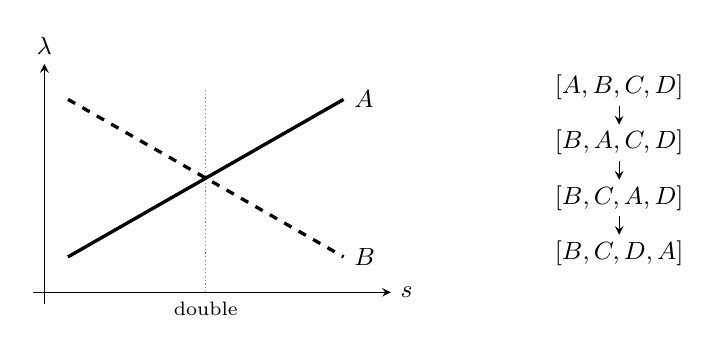
\begin{tikzpicture}[x=1cm,y=1cm,>=stealth,font=\small]
  \draw[->] (0,0.15) -- (4.55,0.15) node[right] {$s$};
  \draw[->] (0.15,0) -- (0.15,3.05) node[above] {$\lambda$};
  \draw[gray,densely dotted] (2.2,0.15) -- (2.2,2.75);
  \draw[very thick] (0.45,0.6) -- (3.95,2.6) node[right] {$A$};
  \draw[very thick,dashed] (0.45,2.6) -- (3.95,0.6) node[right] {$B$};
  \node[font=\scriptsize,below] at (2.2,0.15) {double};

  \node at (7.45,2.75) {$[A,B,C,D]$};
  \node at (7.45,2.05) {$[B,A,C,D]$};
  \node at (7.45,1.35) {$[B,C,A,D]$};
  \node at (7.45,0.65) {$[B,C,D,A]$};
  \draw[->] (7.45,2.52) -- (7.45,2.28);
  \draw[->] (7.45,1.82) -- (7.45,1.58);
  \draw[->] (7.45,1.12) -- (7.45,0.88);
\end{tikzpicture}
\caption{Schematic of a continued pair at an isolated double (left)
and the increasing adjacent-swap schedule on four illustrative ranks
(right). The solid line $A$ changes from lower to upper ordered rank;
the four-rank schedule sends the first label to the last rank. No
numerical eigenvalues or phase durations are represented.}
\label{fig:ang-crossing-cycle}
\end{figure}
